%%%%%%%%%%%%%%%%%%%%%%%%%%%%%%%%%%%%%%%%%%%%%%%%%%%%%%%%%%%%%%%%%%%%%
%
% CSCI 1430 Written Question Template
%
% This is a LaTeX document. LaTeX is a markup language for producing 
% documents. Your task is to fill out this document, then to compile 
% it into a PDF document. 
% You will then upload this PDF to `Gradescope' - the grading system 
% that we will use. Instructions for upload will follow soon.
%
% 
% TO COMPILE:
% > pdflatex thisfile.tex
%
% If you do not have LaTeX and need a LaTeX distribution:
% - Online Tool: https://www.overleaf.com/ (recommended)
% - Departmental machines have one installed.
% - Personal laptops (all common OS): www.latex-project.org/get/
%
% If you need help with LaTeX, please come to office hours. 
% Or, there is plenty of help online:
% https://en.wikibooks.org/wiki/LaTeX
%
% Good luck!
% James and the 1430 staff
%
%%%%%%%%%%%%%%%%%%%%%%%%%%%%%%%%%%%%%%%%%%%%%%%%%%%%%%%%%%%%%%%%%%%%%

\documentclass[11pt]{article}

\usepackage[english]{babel}
\usepackage[utf8]{inputenc}
\usepackage[colorlinks = true,
            linkcolor = blue,
            urlcolor  = blue]{hyperref}
\usepackage[a4paper,margin=1.5in]{geometry}
\usepackage{stackengine,graphicx}
\usepackage{fancyhdr}
\setlength{\headheight}{15pt}
\usepackage{microtype}
\usepackage{times}
\usepackage[shortlabels]{enumitem}
\setlist[enumerate]{topsep=0pt}
% a great python code format: https://github.com/olivierverdier/python-latex-highlighting
\usepackage{pythonhighlight}
\usepackage{amssymb}
\usepackage{multicol}
% setup for todo lists:
\usepackage{enumitem}
\newlist{todolist}{itemize}{2}
\setlist[todolist]{label=$\square$}
\usepackage{pifont}
\newcommand{\cmark}{\ding{51}}%
\newcommand{\done}{\rlap{$\square$}{\raisebox{2pt}{\large\hspace{1pt}\cmark}}%
\hspace{-2.5pt}}


\frenchspacing
\setlength{\parindent}{0cm} % Default is 15pt.
\setlength{\parskip}{0.3cm plus1mm minus1mm}

\pagestyle{fancy}
\fancyhf{}
\lhead{Project 0 Questions}
\rhead{CSCI 1430}
\rfoot{\thepage}

\date{}

\title{\vspace{-1cm}Project 0 Questions}


\begin{document}
\maketitle
\vspace{-2cm}
\thispagestyle{fancy}

\section*{Instructions}
\begin{itemize}
  \item Complete the setup checklist.
  \item 4 questions.
  \item Include code, images, or equations where appropriate.
  \item Please make this document anonymous.
  \item We recommend editing this .tex file in \href{https://www.overleaf.com/}{Overleaf} to ensure the used packages are available. If you use pdfLatex, you may need to import the used packages to maintain the formatting. 
  \item Try to keep your answers within the given space. If you really need to, please add a page break after any answer that has gone over the page. On upload, \textbf{Gradescope will ask you to assign question numbers to your pages}.
  \item When you are finished, compile this document to a PDF and submit it directly to Gradescope.
    
\end{itemize}

\section*{Setup Checklist (Graded)}

For each of the following, complete the task and check the box to mark it as done.
\begin{todolist}
    \item[\done] This is an example of a checked box
    \item Read the GitHub tutorial \href{https://docs.google.com/document/d/1Hli-42Tv91tnghbxW4Pn44aGGeV9MMb4NgIktg9jN-U/edit?usp=sharing}{here}.
    \item Create a GitHub account, if you don't have one.
    \item Join the \href{https://www.gradescope.com/}{Gradescope} course.
    \item Join the course \href{https://piazza.com/}{Piazza}.
    \item Compile and read the included Python tutorial.
    \item Set up python environment and virtual environment.
    \item Set up an editing environment (VSCode), get it to use your python virtual environment, and know how to debug within it by setting breakpoints.
\end{todolist}

\section*{Questions}

\paragraph{Q1:} Please find and read the course collaboration policy on the \href{http://cs.brown.edu/courses/csci1430/}{course website} and mark whether each of the following scenarios violates the policy. 

\emph{LaTeX:} To fill in boxes, replace `\textbackslash square' with `\textbackslash blacksquare' for your answer.

\begin{enumerate}[(a)]
\item 
Another CSCI1430 student looking at your code to help you debug, after you have spent time trying to tackle the bug or have come to TA office hours/Piazza.

\begin{tabular}[h]{ll}
$\square$ & Acceptable \\
$\square$ & Violation \\
\end{tabular}

\item 
Using the result images from another student's code for your write up because your code is broken.

\begin{tabular}[h]{ll}
$\square$ & Acceptable \\
$\square$ & Violation \\
\end{tabular}

\item 
Googling third party sites to clarify concepts for written and code assignments, with proper citation.

\begin{tabular}[h]{ll}
$\square$ & Acceptable \\
$\square$ & Violation \\
\end{tabular}

\item 
A student who has previously taken the course and is not currently a TA sharing code with you to help you get through a bug.

\begin{tabular}[h]{ll}
$\square$ & Acceptable \\
$\square$ & Violation \\
\end{tabular}

\end{enumerate}



%%%%%%%%%%%%%%%%%%%%%%%%%%%%%%%%%%%


%%%%%%%%%%%%%%%%%%%%%%%%%%%%%%%%%%%

% Please leave the pagebreak
\pagebreak

\paragraph{Q2:}
Computer vision is all around us, sometimes in surprising ways. 
\begin{enumerate}[(a)]

\item
If you could have any computer vision related superpower---there are no limitations---what would it be?

\item
How would you use your superpower? 

\item Find a recent example (past 6 months or so) of a controversial real world use of computer vision. What caused the controversy?

Please cite a source. Extra credit for unique examples!
\end{enumerate}

%%%%%%%%%%%%%%%%%%%%%%%%%%%%%%%%%%%
\paragraph{A2:} Your answer here.
% Uncomment the stencil below and fill in your solution.

% \begin{enumerate}[(a)]

% \item 

% \item 

% \item 

% \end{enumerate}

%%%%%%%%%%%%%%%%%%%%%%%%%%%%%%%%%%%


% Please leave the pagebreak
\pagebreak
\paragraph{Q3:} We wish to set all pixels that have a value of 10 or less to 0, to remove camera sensor noise. However, our code is slow when run on a database with 1000 grayscale images.

\emph{Image:} \href{grizzlypeakg.png}{grizzlypeakg.png}

\begin{python}
from skimage import io

A = io.imread('grizzlypeakg.png')
(m1,n1) = A.shape
for i in range(m1):
    for j in range(n1):
        if A[i,j] <= 10 :
            A[i,j] = 0       
\end{python}

How could we speed it up? Please include your code. \\

%%%%%%%%%%%%%%%%%%%%%%%%%%%%%%%%%%%
\paragraph{A3:} Your answer here.



%%%%%%%%%%%%%%%%%%%%%%%%%%%%%%%%%%%

% Please leave the pagebreak
\pagebreak
\paragraph{Q3.2:} What factor speedup would we receive over 1000 images? Please measure it and include your code.

Ignore file loading; assume all images are equal resolution; don't assume that the time taken for one image $\times1000$ will equal $1000$ image computations, as single short tasks on multitasking computers often take variable time.

\emph{Note: Running the slow code on 1000 images might take 45 minutes or more! You can compute the factor on just 10 images. For the sped-up version, you might need to compute the time on more images to receive a more reliable estimate of the average time. Be sure to compensate for the number of images computed against in your speedup factor.}

%%%%%%%%%%%%%%%%%%%%%%%%%%%%%%%%%%%
\paragraph{A3.2:} Your answer here.



%%%%%%%%%%%%%%%%%%%%%%%%%%%%%%%%%%%

% Please leave the pagebreak
\pagebreak
\paragraph{Q3.3:} Next, we wish to operate on color images. How does your speeded-up version from Q3.2 change for color images? Please implement and measure it, report the speed factor change, and include your code.

\emph{Note: We will change the value in each color channel; we do not wish to convert the image to grayscale.}

\emph{Image:} \href{grizzlypeak.jpg}{grizzlypeak.jpg}

%%%%%%%%%%%%%%%%%%%%%%%%%%%%%%%%%%%
\paragraph{A3.3:} Your answer here.



%%%%%%%%%%%%%%%%%%%%%%%%%%%%%%%%%%%

% Please leave the pagebreak
\pagebreak
\paragraph{Q4:} We wish to reduce the brightness of an image by editing the values in its matrix. But, when trying to visualize the result, we see some ``errors''.

\emph{Image:} \href{gigi.jpg}{gigi.jpg}

\begin{python}
from skimage import io
import matplotlib.pyplot as plt
import numpy as np

I =  io.imread('gigi.jpg').astype(np.float32)
I = I - 50
plt.imshow( I )
plt.show()
\end{python}

What is incorrect with this approach? How can it be fixed while maintaining the same intended brightness reduction? Please include your code and result image.

%%%%%%%%%%%%%%%%%%%%%%%%%%%%%%%%%%%
\paragraph{A4:} Your answer here.

% Example image inclusion; replace with your result image:
% 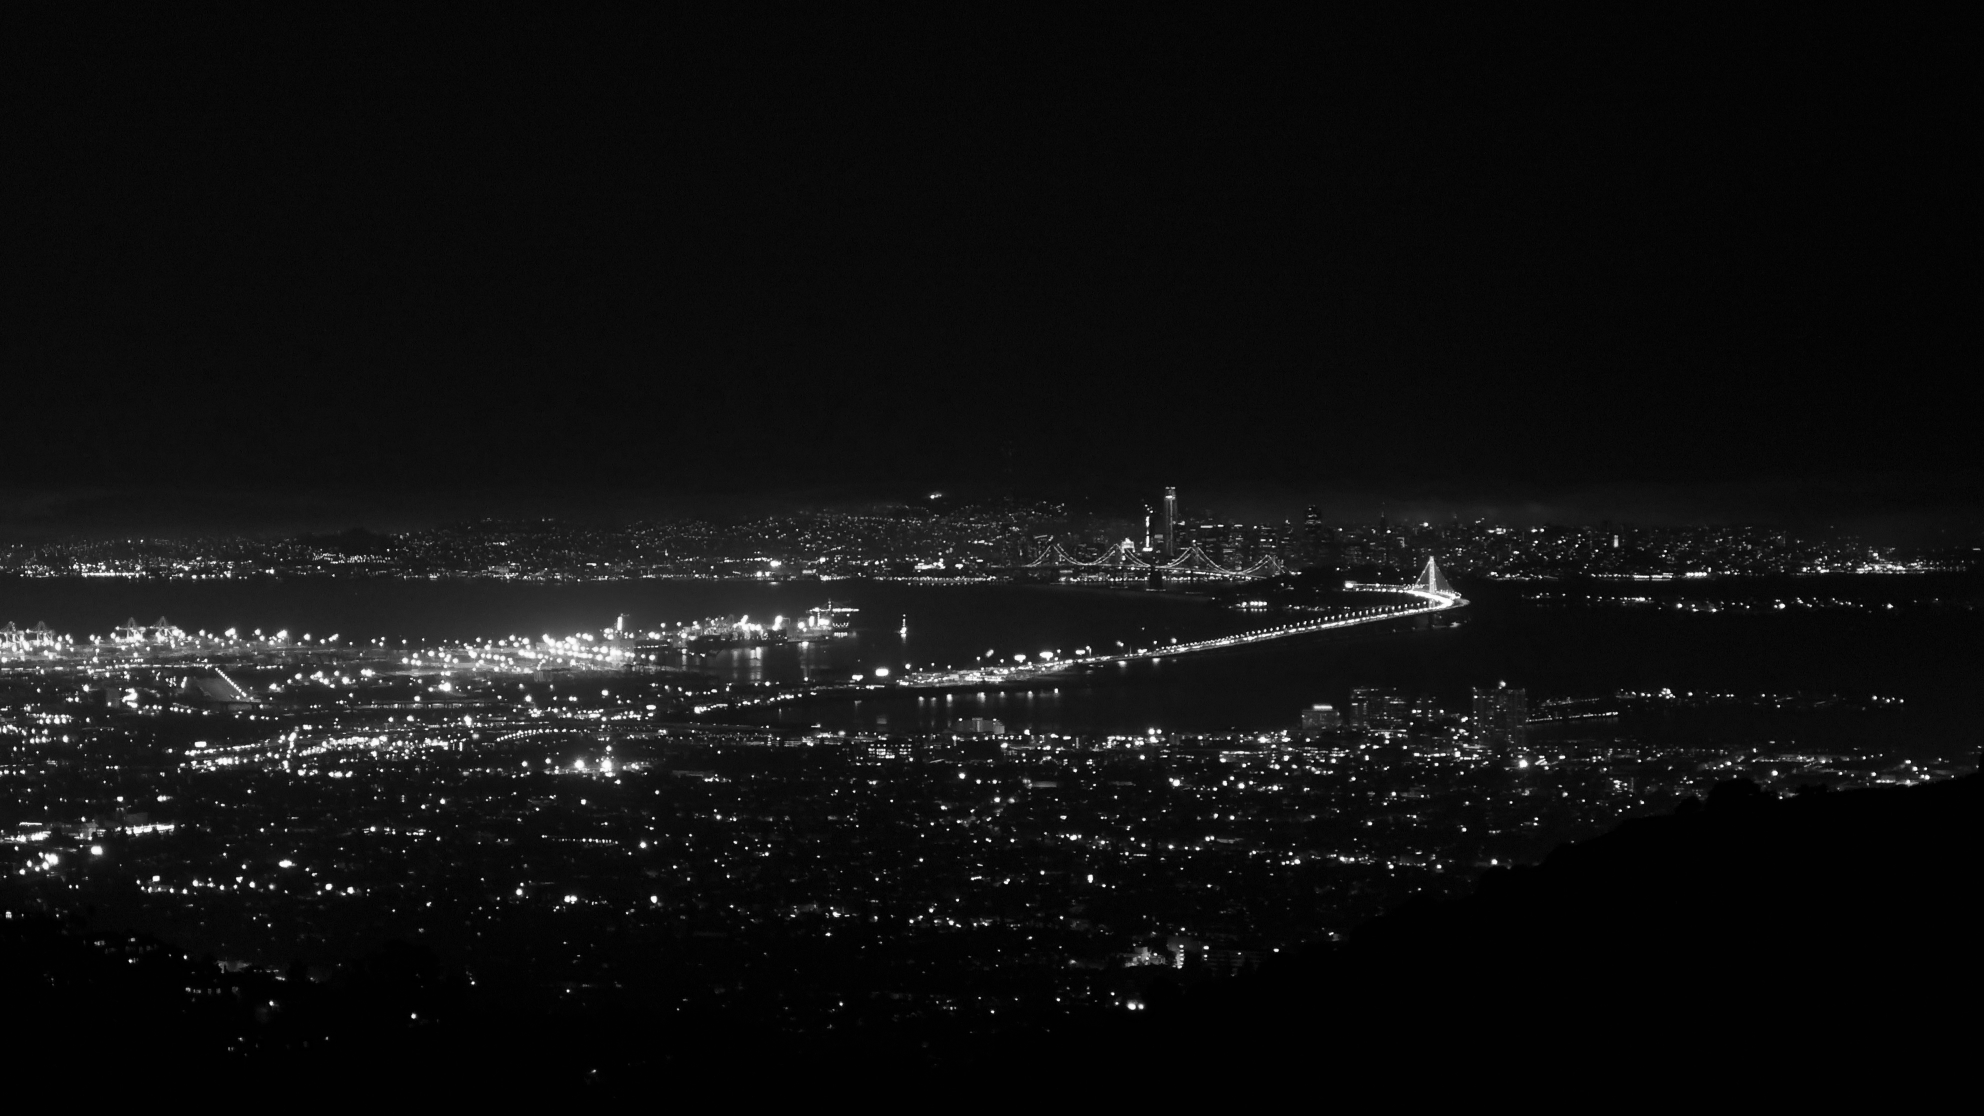
\includegraphics[width=\textwidth]{grizzlypeakg.png}


%%%%%%%%%%%%%%%%%%%%%%%%%%%%%%%%%%%

\end{document}
